% !TEX TS-program = XeLaTeX
\documentclass[conference]{IEEEtran}
\IEEEoverridecommandlockouts
% The preceding line is only needed to identify funding in the first footnote. If that is unneeded, please comment it out.
\usepackage{cite}
\usepackage{amsmath,amssymb,amsfonts}
\usepackage{algorithmic}
\usepackage{graphicx}
\usepackage{textcomp}
\usepackage{booktabs} 
\usepackage{subfigure}
\def\BibTeX{{\rm B\kern-.05em{\sc i\kern-.025em b}\kern-.08em
    T\kern-.1667em\lower.7ex\hbox{E}\kern-.125emX}}
\begin{document}

\title{Artificial Intelligence Cource Project\\
{\footnotesize CS410
}
}

\author{
\IEEEauthorblockN{ Ruijie Wang}
\IEEEauthorblockA{
\textit{515021910338}\\
Wjerry5@sjtu.edu.cn}

}

\maketitle
\begin{abstract}
This document is a model and instructions for \LaTeX.
This and the IEEEtran.cls file define the components of your paper [title, text, heads, etc.]. *CRITICAL: Do Not Use Symbols, Special Characters, Footnotes, 
or Math in Paper Title or Abstract.
\end{abstract}

\section{introduction}

\section{method}
\subsection{Data Processing}
Since the given dataset is a large p small n problem, dimensionality reduction is required at first. In this part, we will introduce two dimensionality reduction methods: PCA and Autoencoder. Later we compare both their performances and their individual result under different dimension using a same SVM  classifier.

\subsubsection{PCA}
Principal components analysis(PCA)\cite{PCA} aims to perform a linear mapping of the data to a lower-dimensional space in such a way that the variance of the data in the low-dimensional representation is maximized. Suppose we are given data matrix $X$ with size $n\times p$, where n is the quality of sampling and p is the dimension of feature. The PCA algorithm is shown as follow:
\begin{itemize}
\item Normalize the data : $x=x-\sum_i^N x_i$;
\item Calculate the covariance matrix $C=\frac{X^T X}{n-1}$. Then diagonalize it : $C=V L V^T$, where $V$ is the matrix of eigenvectors and $L$ is diagonal matrix with eigenvalues $��_i$ .
\item Choose $d$ rows ,the sum of whose variance reach some percentage of original variance. The criterion should be followed Eq(\ref{pac_1}).

\begin{centering}
\begin{equation}
\frac{\sum^d_i \lambda_i}{\sum^n_i \lambda_i} \ge Threshold
\label{pac_1}
\end{equation}
\end{centering} 
\end{itemize}

The final $p$ is determined by $Threshold$. PCA is based on the idea that the feature has large variance but the noise has low variance. 

\subsubsection{Autoencoder}An autoencoder neural network is an unsupervised learning algorithm that applies back propagation, setting the target values to be equal to the inputs. The structure of autoencoder is show as Fig(\ref{auto_1}):
\begin{figure}[!ht]
  \centering
   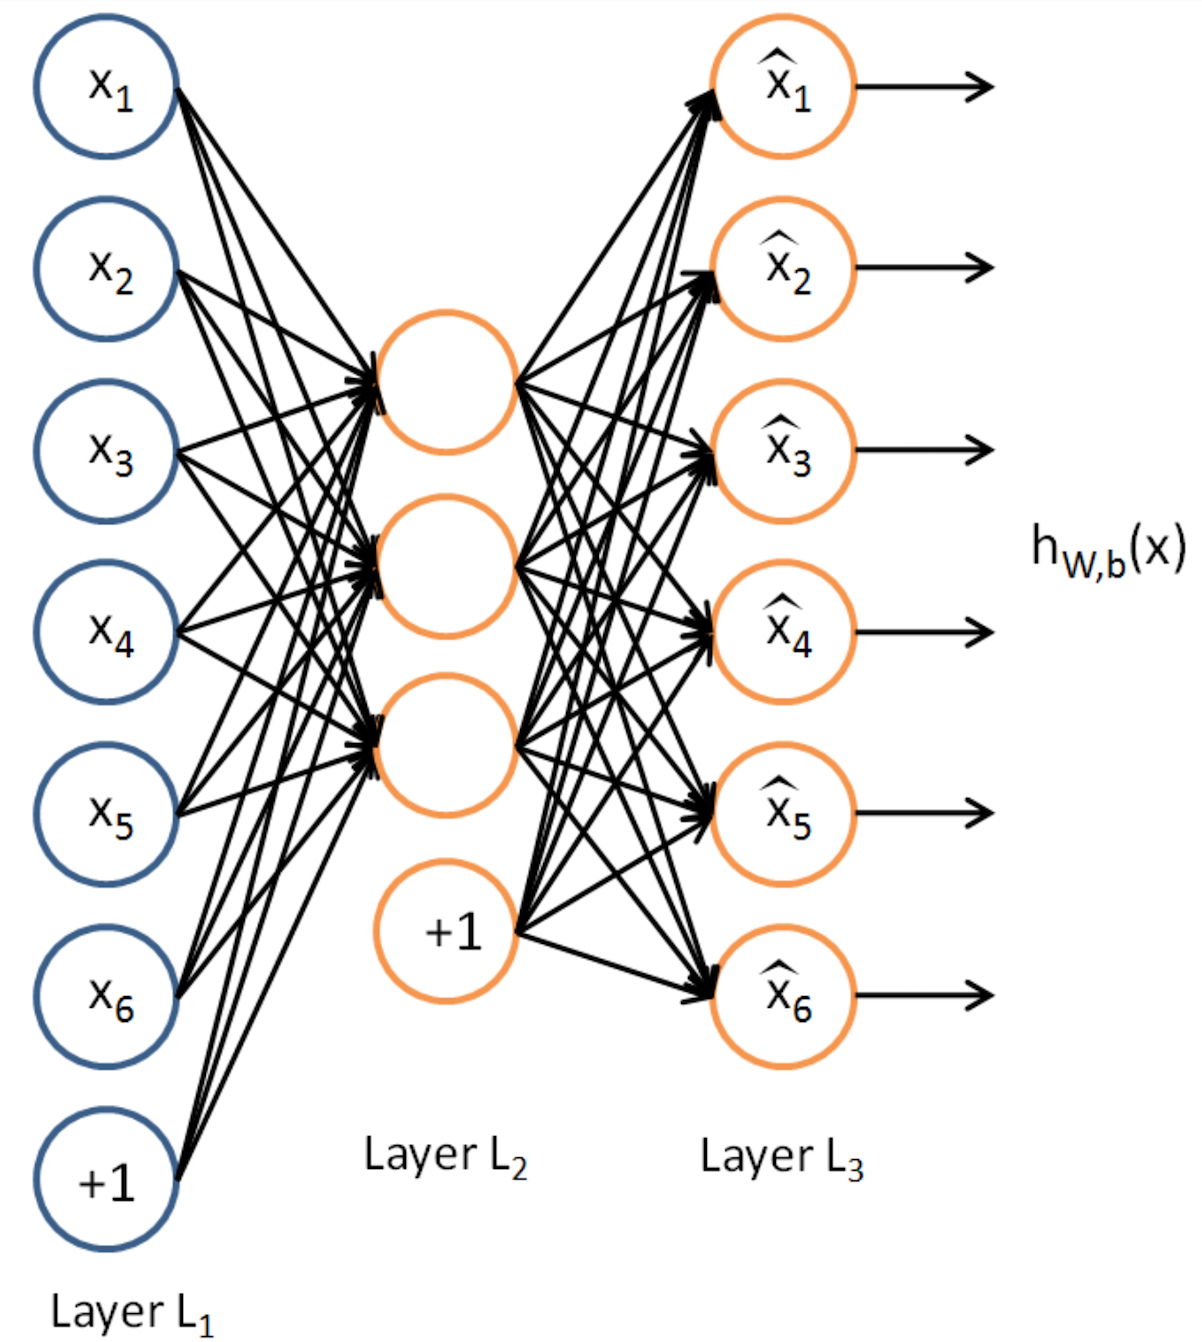
\includegraphics[width=0.5\textwidth ,height=6cm]{../figs/auto_1.png}
   \caption{structure of autoencoder}
   \label{auto_1}
   \centering
\end{figure}

Now suppose we have  a set of unlabeled training examples $X=[x_1,x_2,x_3,\dots]$, we want $X=H_{W,b}(X)$. Then the lower-dimension output of hidden layer L2 is the encoder of the raw data. This output is a nonlinear dimensionality reduction, which may overcome the weakness of PCA that it is only a linear dimensionality reduction method.
\subsection{Classical Methods}


\subsubsection{Logistic Regression}
Logistic regression is a  classical  supervised linear classifier. Generally speaking, logistic regression firstly calculates the boundary among different classes, then it  can predict the possibility of test data class based on the calculated  data boundary.  

Suppose now that we are given all of the training dataset annotated with labels, while $\mathbf{x}$ denotes the feature vector and $\mathbf{Y}$ denotes label, then the calculated class possibility is defined as Eq(\ref{lr_1}):

\begin{centering}
\begin{equation}
P(Y=y_i|x_i)=\frac{e^{\omega x_i +b}}{1+\sum_i e^{\omega x_i +b}} 
\label{lr_1}
\end{equation}

\end{centering}
where $\omega$ denotes the regression weights and $b$ denotes the regression bias. Based on the labels training data, we can determine the value of $\omega$ and $b$ using Maximum Likelihood Estimation(MLE) method. Assume $h_\omega(x_i)$ denoting the possibilities, the log likelihood function is defined as Eq(\ref{lr_2}):

\begin{centering}
\begin{equation}
L(\omega)=\sum^N_i[y_i logh_\omega(x_i)+(1-y_i) log(1-h_\omega(x_i))]
\label{lr_2}
\end{equation}

\end{centering}

Various gradient-based optimize algorithm can be used to determine the value of $\omega$ and $b$. In our work, we use logistic regression in both multiple classification task and binary classification task and we compare its performance under various optimization and regularization methods.

\subsection{Deep Learing Based Methods}
Deep learning\cite{Deeplearning} has been shown as a successful machine learning method for a variety of tasks. In our work, we use a deep neural network with fully-connected multilayer structure both on PCA-processed data and on raw data with \textbf{greedy layer-wise pre training}. Besides, we add L2 regularization in each fully-connected layer to avoid overfitting and control the model complexity.
\subsubsection{network structure} Since the features do not have any locality or direct relationship, we don��t use convolutions.\\

\begin{itemize}
\item \textbf{nn on pca-processed data}\\
In this model, firstly we use pca-processed data (500-dimension) as our network input. Then we add hidden layer1(256-dimension), hidden layer2(512-dimension), hidden layer3(256-dimension), finally a output layer.  The structure is shown as Fig(\ref{nn_1}) network \romannumeral1. 
For weight initialization, we initialize each neurons weight vector as a random vector sampled from a multi-dimensional gaussian. For bias initialization, we set the bias vectors all to $0$. We initialize our weight with the consideration that the size of our network is limited and it can be trained easily according to the network \romannumeral2.

\item \textbf{nn on raw data}\\
In this model, we use the raw data as the network inputs. Then we add hidden layer1(8192-dimension), hidden layer2(512-dimension), hidden layer3(128-dimension), finally a output layer.  The structure is shown as Fig(\ref{nn_1}) network \romannumeral2. Since we did not use the low-dimension data, the training become much harder according to out experiment. So the network initialization is very import. We use greedy layer-wise pre training , which is a pre-train method based on the idea of autoencoder, to initialize the network. 
\end{itemize}

\begin{figure}[!ht]
\centering
   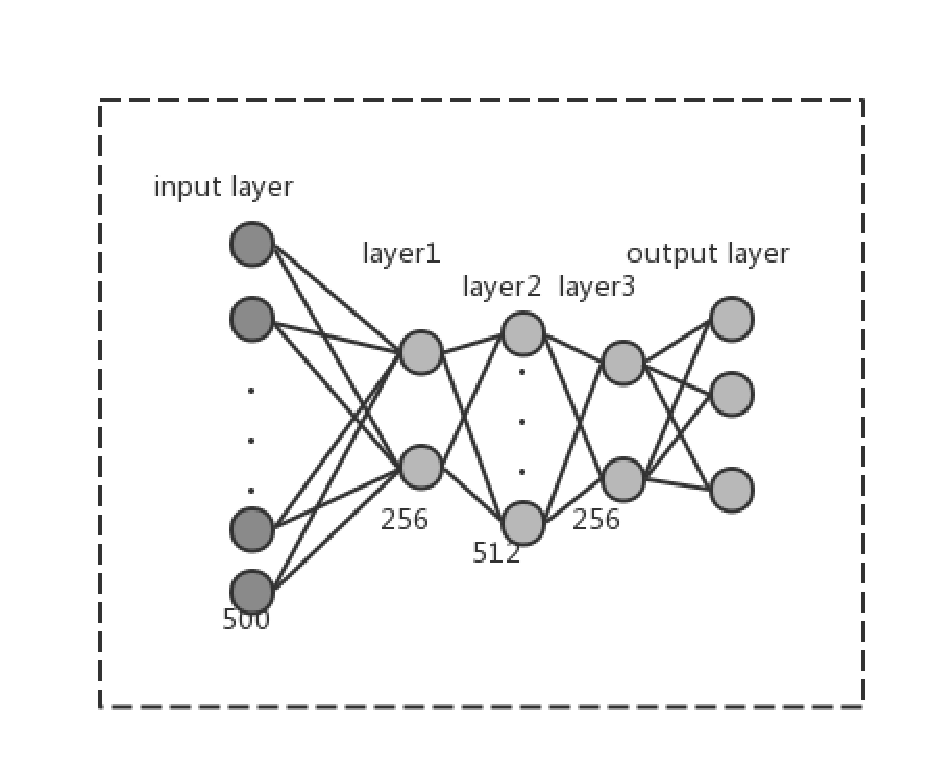
\includegraphics[width=0.24\textwidth]{../figs/nn_pca.pdf}
   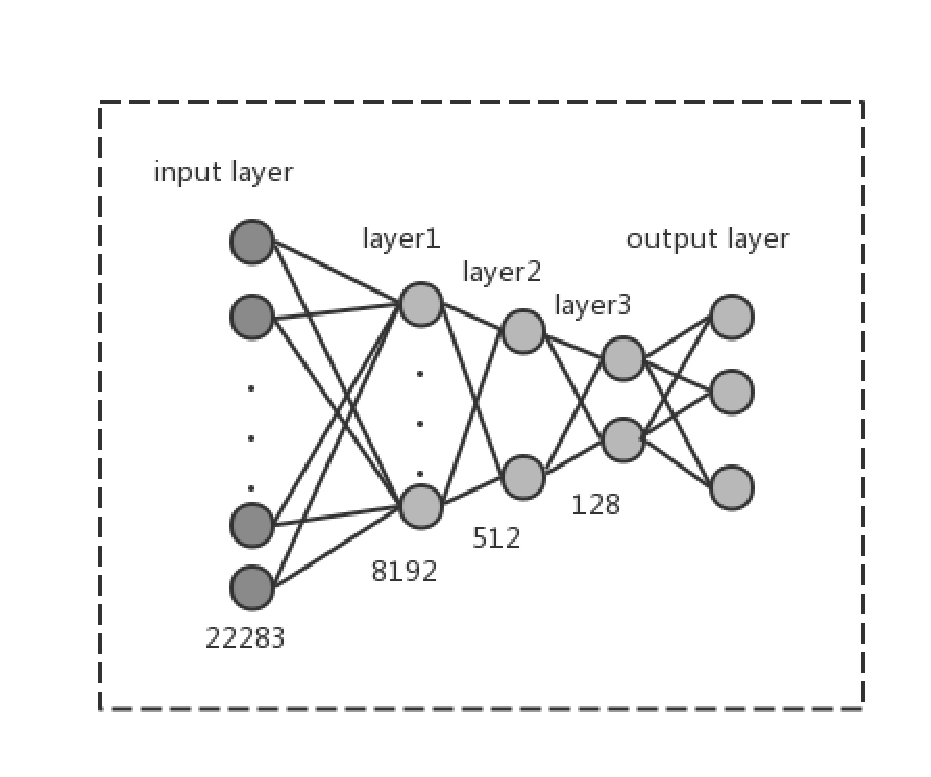
\includegraphics[width=0.24\textwidth]{../figs/nn_raw.pdf}
   \caption{a.network \romannumeral1;  b, network \romannumeral2; }
   \label{nn_1}
\centering
\end{figure}

\subsubsection{Regularization}
We use L2 regularization in each fullt-connected layer.It can be implemented by penalizing the squared magnitude of all parameters directly in the objective. For every weight $w$ in the network, we add the term $1/2��w$ to the objective, where �� is the regularization strength. This can help control the capacity of neural networks to prevent overfitting.

Furthermore, we employ Dropout\cite{Dropout} to prevent overfit- ting. While training, dropout is implemented by only keep- ing a neuron active with some probability p, or setting it to zero otherwise.

\subsubsection{Pre-train}
In network \romannumeral2, the training get very hard because of the high dimension of the network. We use \textbf{greedy layer-wise pre training} to pre-train. It will determine the initial weights of each layer layer by layer with the idea of autoencoder. Since each layer has been local optimal solution, the training get much easier .

More specifically, to determine weights of first hidden layer, we use the network shown as Fig(\ref{auto_1}). Once we get $X=h_{\omega,b}(X)$, it means the hidden layer can encode the input properly, at the same time it can pass these extracted feature to the following layer. Seemingly, when we initialize the second hidden layer, we use the output of the first hidden layer as the input of network in Fig(\ref{auto_1}). Thus we can determine all the weights. The process is show as Fig(\ref{pretrain_1}). The network \romannumeral4  in  Fig(\ref{pretrain_1}) is we want, so to determine the 3 layers weights, we use network \romannumeral1-network \romannumeral3 (which are same as  Fig(\ref{auto_1})) to train them.

\begin{figure}[!ht]
\centering
   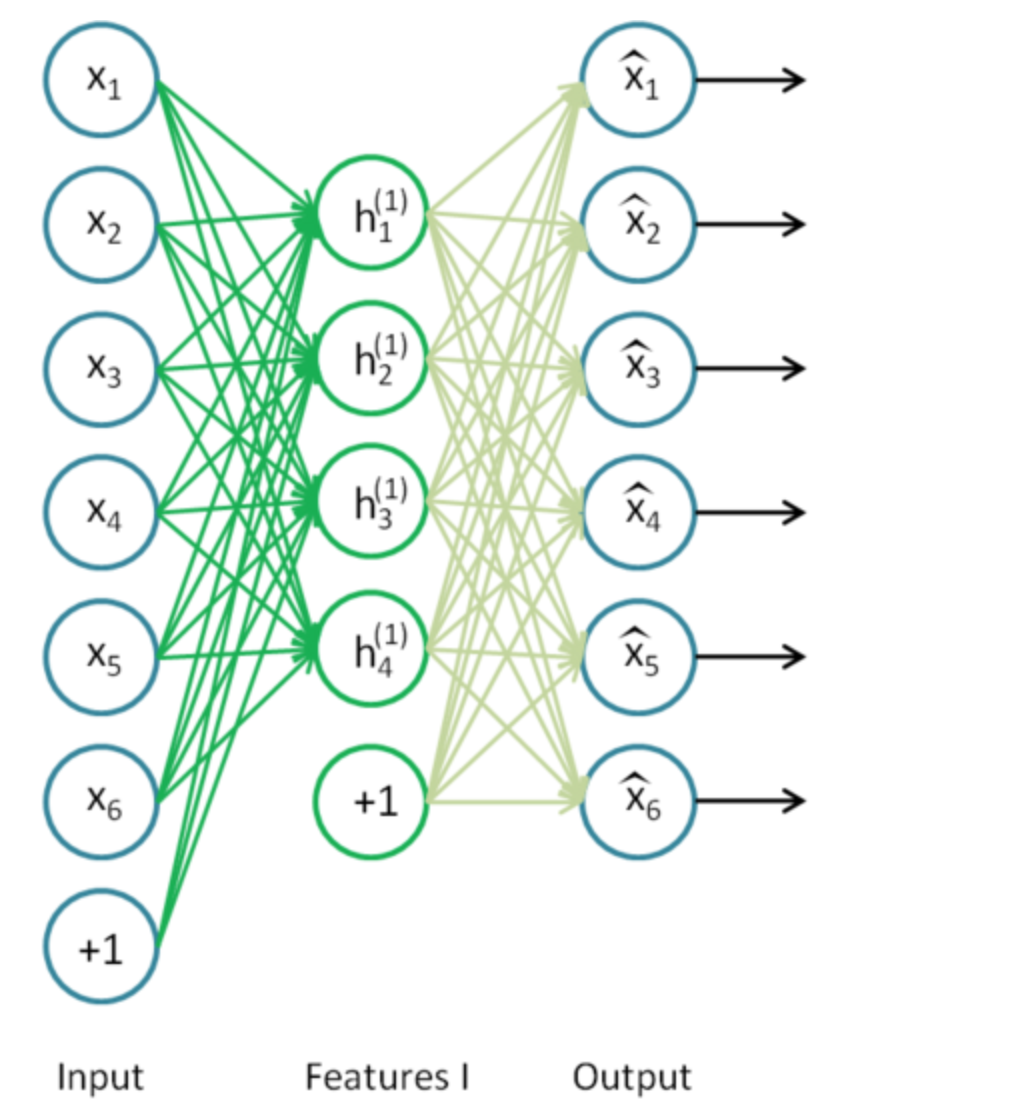
\includegraphics[width=0.24\textwidth,height=3cm]{../figs/pretrain1.png}
   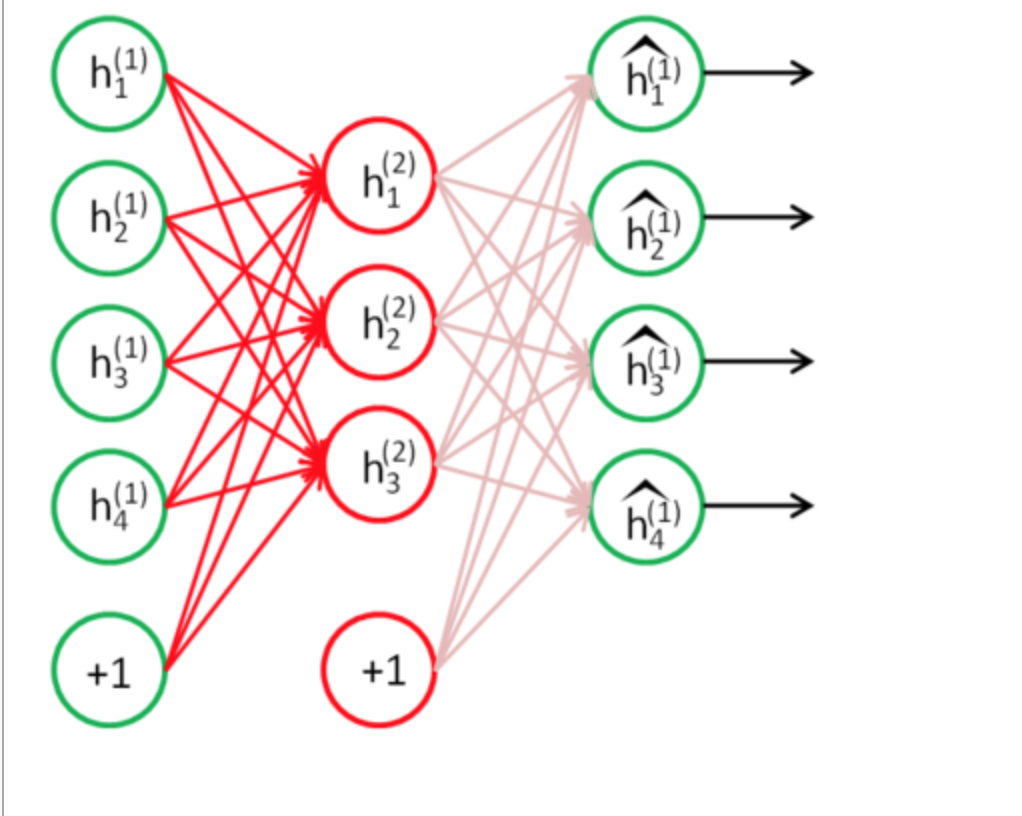
\includegraphics[width=0.24\textwidth,height=3cm]{../figs/pretrain2.png}
   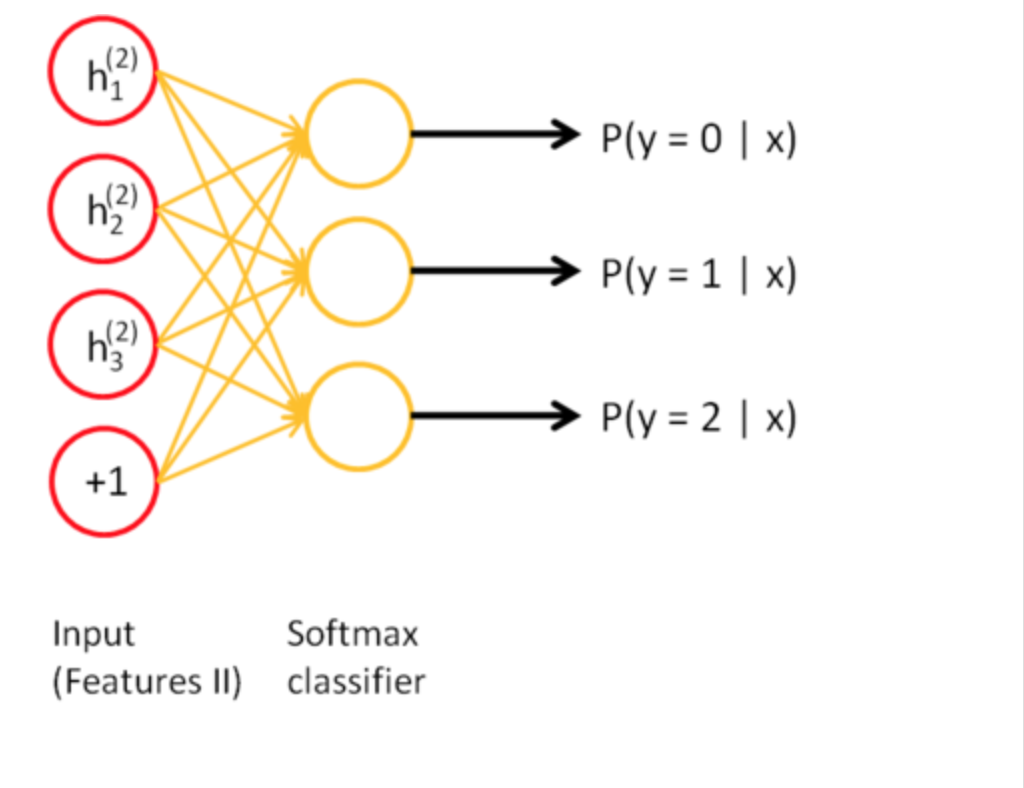
\includegraphics[width=0.24\textwidth,height=3cm]{../figs/pretrain3.png}
   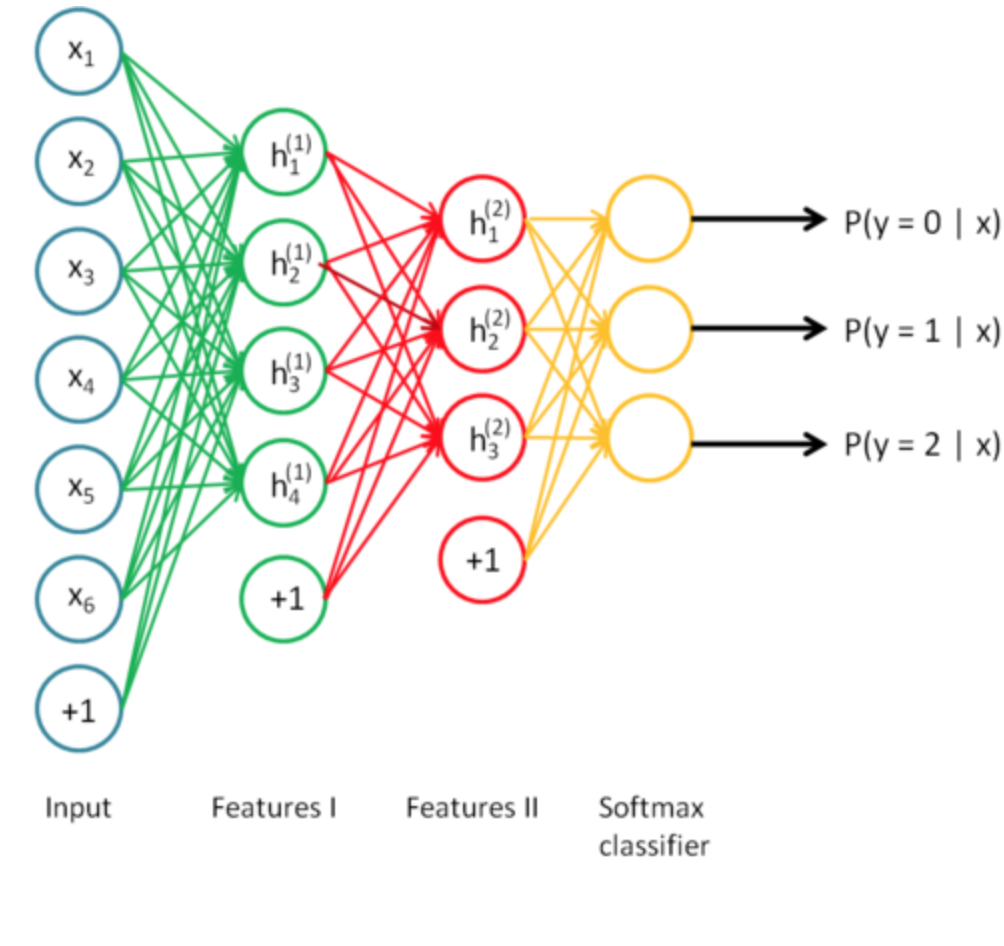
\includegraphics[width=0.24\textwidth,height=3cm]{../figs/pretrain4.png}
   \caption{a.network \romannumeral1;  b, network \romannumeral2; c, network \romannumeral3; d, network \romannumeral4}
   \label{pretrain_1}
\centering
\end{figure}

\section{experiment}
\subsection{Label Selection} Besides, we visualize the given data with selected labels into 2-D figure using PCA method, which is shown in Fig(\ref{distribution_1}). By observation, data with Bio-7 label, Material-2 label and Disease-16 have clear boundary while it is very hard to identify the data with Sex-2 label in 2-D space.

\begin{figure}[!ht]
\centering
   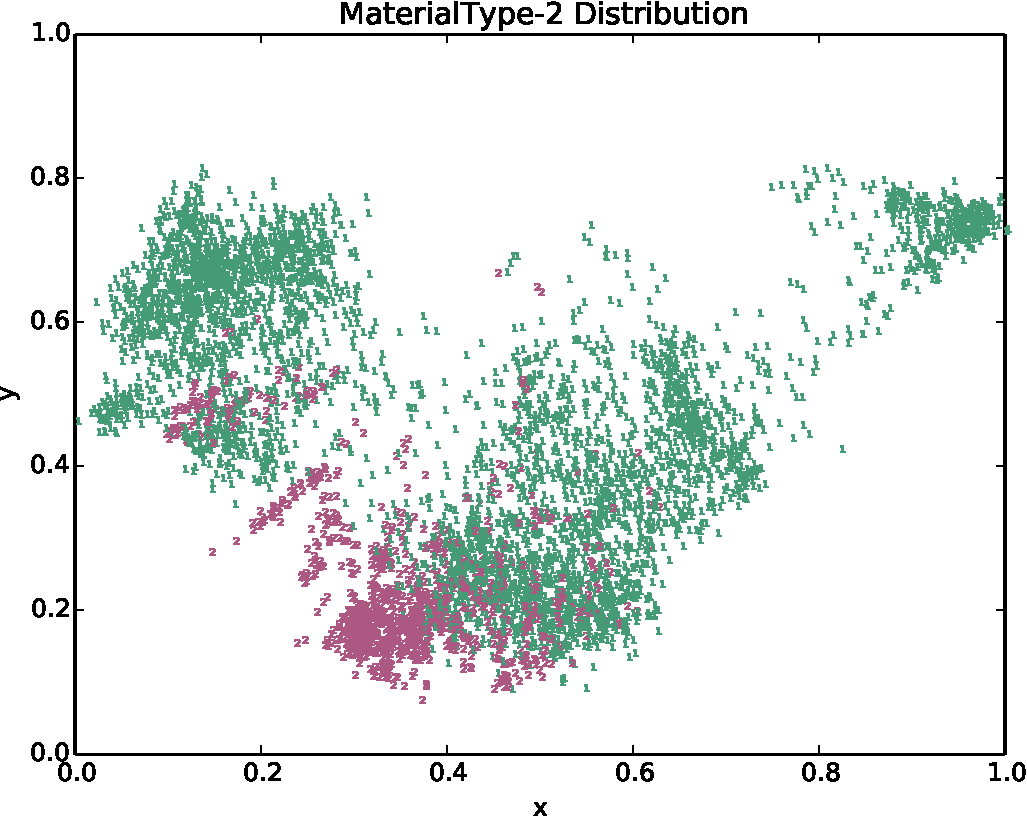
\includegraphics[width=0.24\textwidth]{../figs/Material-2.pdf}
   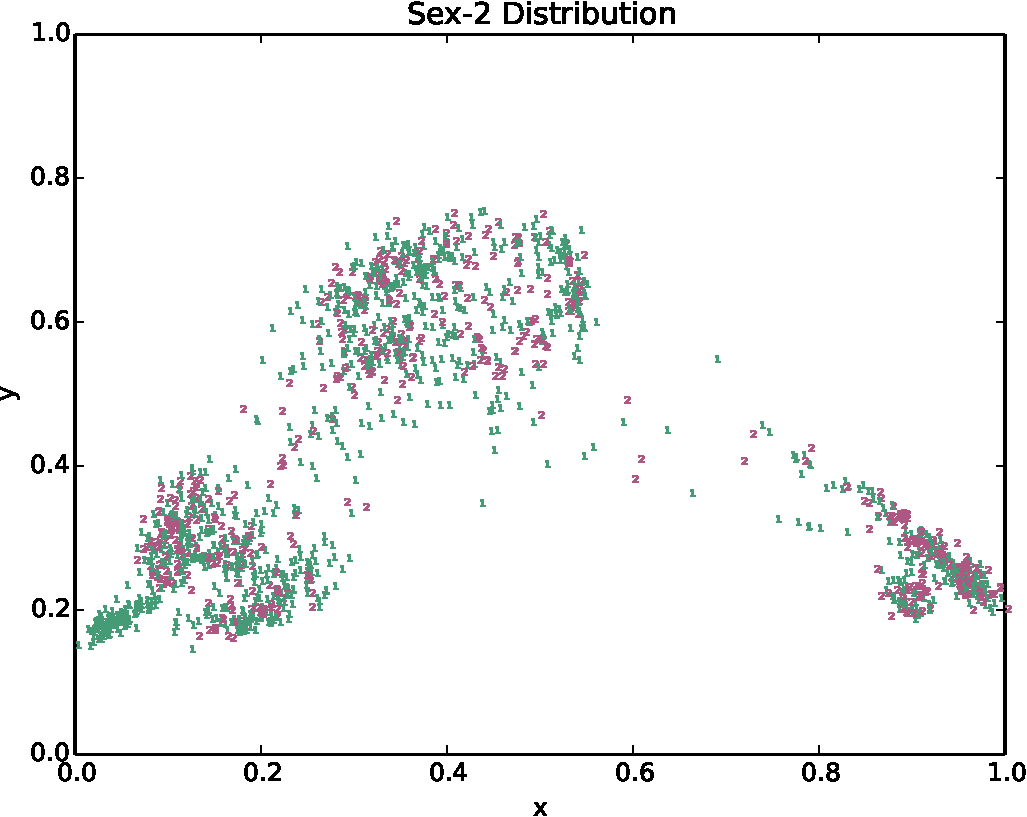
\includegraphics[width=0.24\textwidth]{../figs/Sex-2.pdf}
   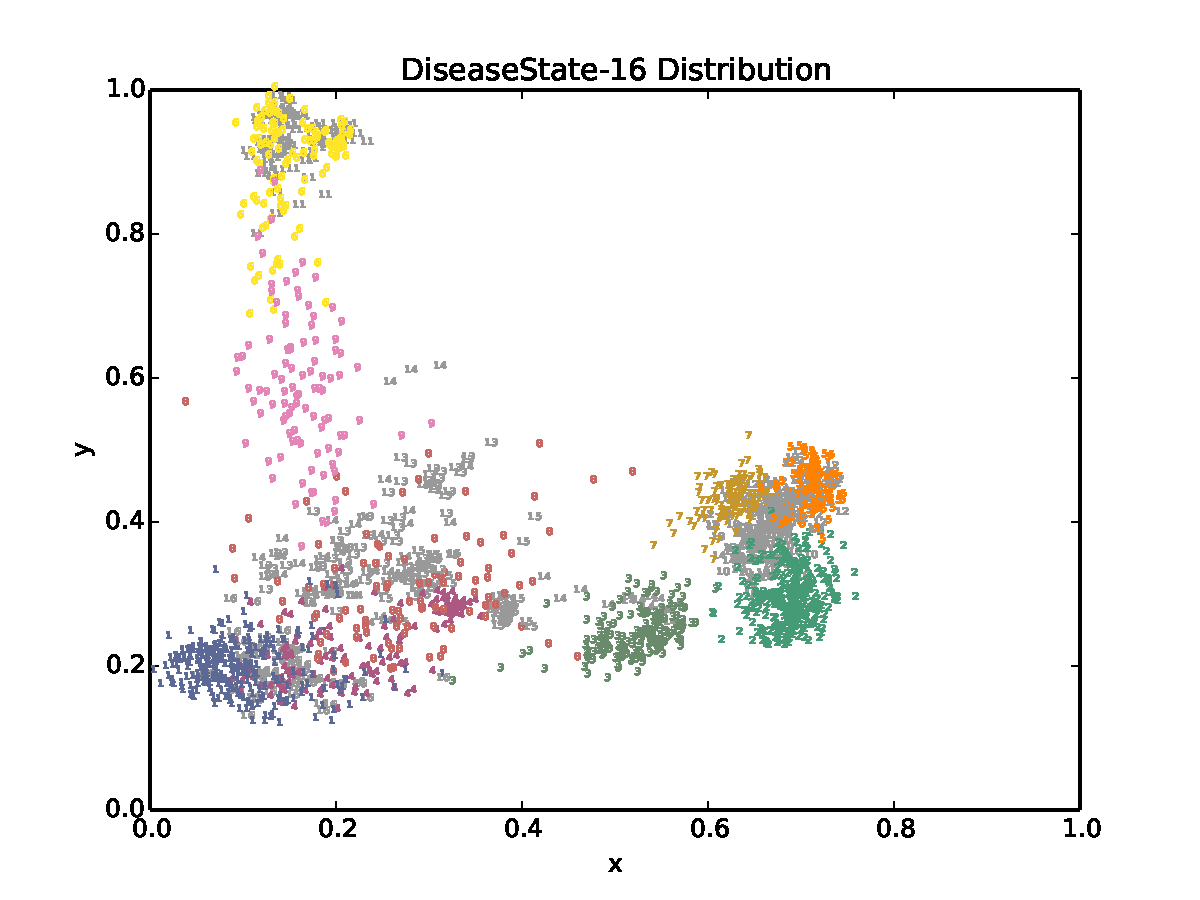
\includegraphics[width=0.24\textwidth]{../figs/Disease-16.pdf}
   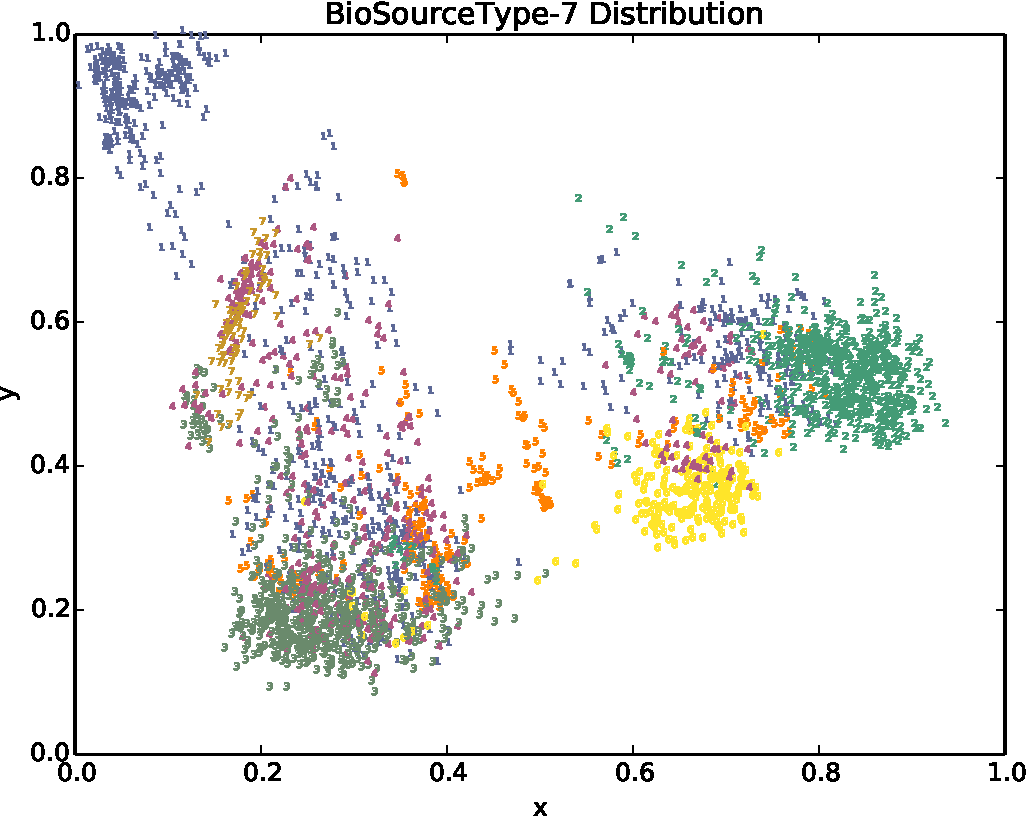
\includegraphics[width=0.24\textwidth]{../figs/Bio-7.pdf}
   \caption{a.Material-2 Distribution;  b, Sex-2 Distribution2; c, Disease-16 Distribution; d,Bio-7 Distribution}
   \label{distribution_1}
\centering
\end{figure}
\section{result}
\subsection{Logistic Regression} 
We apply logistic regression to four task. Besides, we try different regularization method and solver  with different regularization strength C . We want to choose the best parameter settings and compare the preformence of different regularization method and solver. The result with the change of C is shown as Fig(\ref{lr_result1}).It can be seen that the performance of LR did not vary too much with the change of C, which may mean the data distribution is ideal and the  regularization of this model is not necessary.

\begin{figure}[!ht]
\centering
   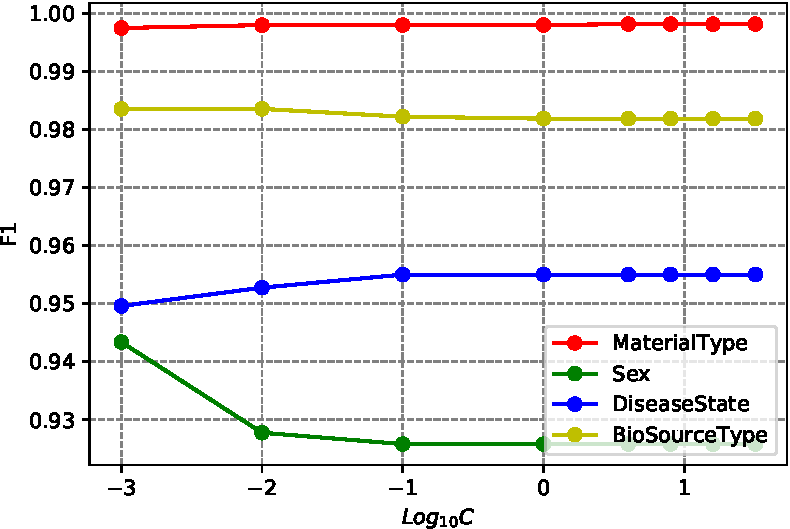
\includegraphics[width=0.4\textwidth]{../figs/LR_C.pdf}
   \caption{The performance of LR in 4 tasks with different regularization strength.}
   \label{lr_result1}
\centering
\end{figure}

And the best results on 4 tasks with selected parameters is shown in Table(\ref{lr_result2}).

\begin{table}[tbp]
		\centering
		\begin{tabular}{l|cccc}
			\toprule
			{Label Type} & $F_1 (\%)$ & C &solver &penalty \\
			\midrule
			{\textit{MaterialType}}&99.86 & 4 &lbfgs & l2\\
			{\textit{Sex}}		& 94.96 & 0.001    &sag & l2 \\
			{\textit{DiseaseState}}& 95.72 & 0.001 &lbfgs & l2\\
			{\textit{BioSourceType}}& 98.42 & 0.01 &lbfgs & l2\\
			\bottomrule	
		\end{tabular}
		
		\caption{Best results and parameter settings for Logistic Regression. }
		\label{lr_result2}
	\end{table}




\subsection{Deep Learning based Method}

\subsubsection{ nn on pca-processed data}
At first we try deep neural network on   pca-processed data. The dimension is 500, and the network is shown in Fig{\ref{nn_1}). Besides,  we use L2 regularization and dropout to avoid overfitting. The dropout rate is 0.50. In the end, we use batch normalization in each layer and it greatly improves the performance. The results and selected parameters are shown in Table(\ref{nnpca_result}).

	\begin{table}[tbp]
		\centering
		\begin{tabular}{l|cccc}
			\toprule
			{Label Type} & $F_1 (\%)$ & learning rate &$batch size$  \\
			\midrule
			{\textit{MaterialType}}&99.30 & 0.001 &32\\
			{\textit{Sex}}		& 92.92 & 0.001    &50 \\
			{\textit{DiseaseState}}& 94.38 & 0.001 &32\\
			{\textit{BioSourceType}}& 95.87 & 0.001 &16\\
			\bottomrule	
		\end{tabular}
		
		\caption{Best results and parameter settings for nn model on pca data. }
		\label{nnpca_result}
	\end{table}
	
Besides, we visualize the training process of Sex and Bio tasks with the change of learning. It is shown in Fig(\ref{lr_result}), and it can be seen $lr=0.001$ is the best result in four task. 

\begin{figure}[!ht]
\centering
   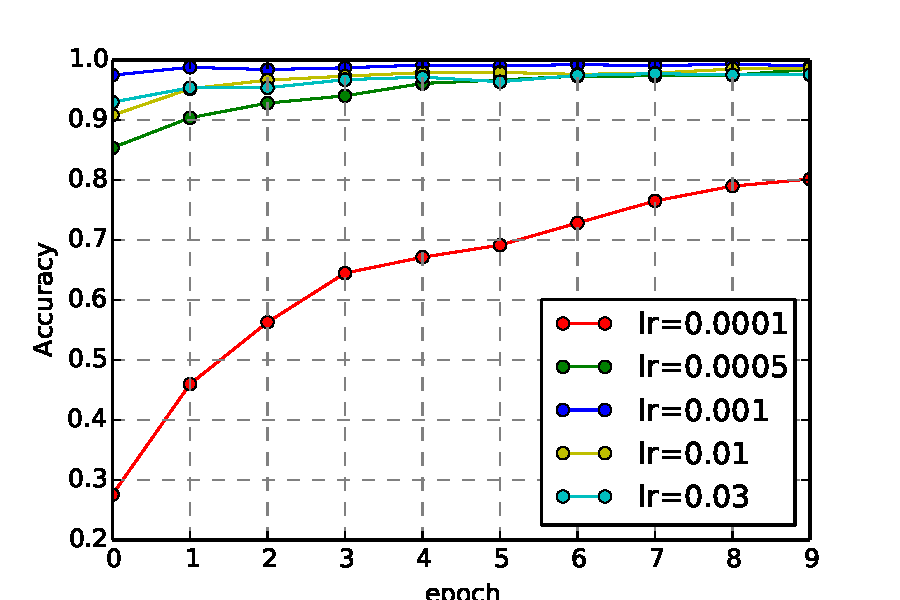
\includegraphics[width=0.24\textwidth]{../figs/lr_acc_bio.pdf}
   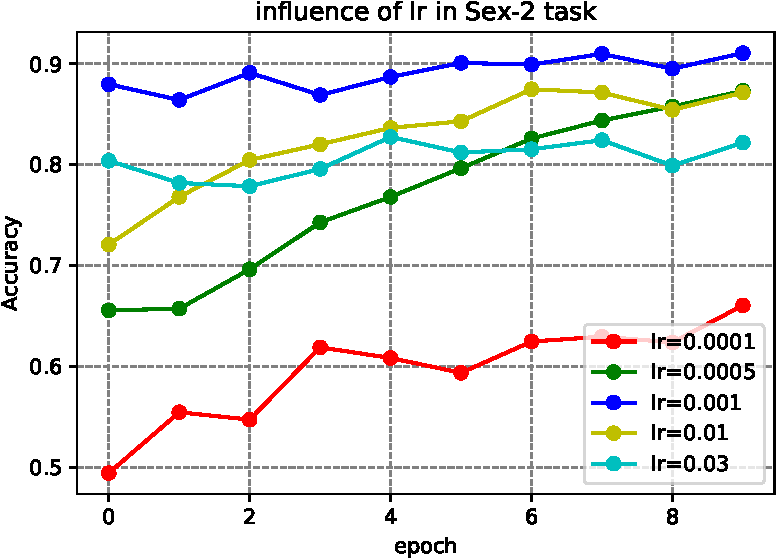
\includegraphics[width=0.24\textwidth]{../figs/lr_acc_sex.pdf}
   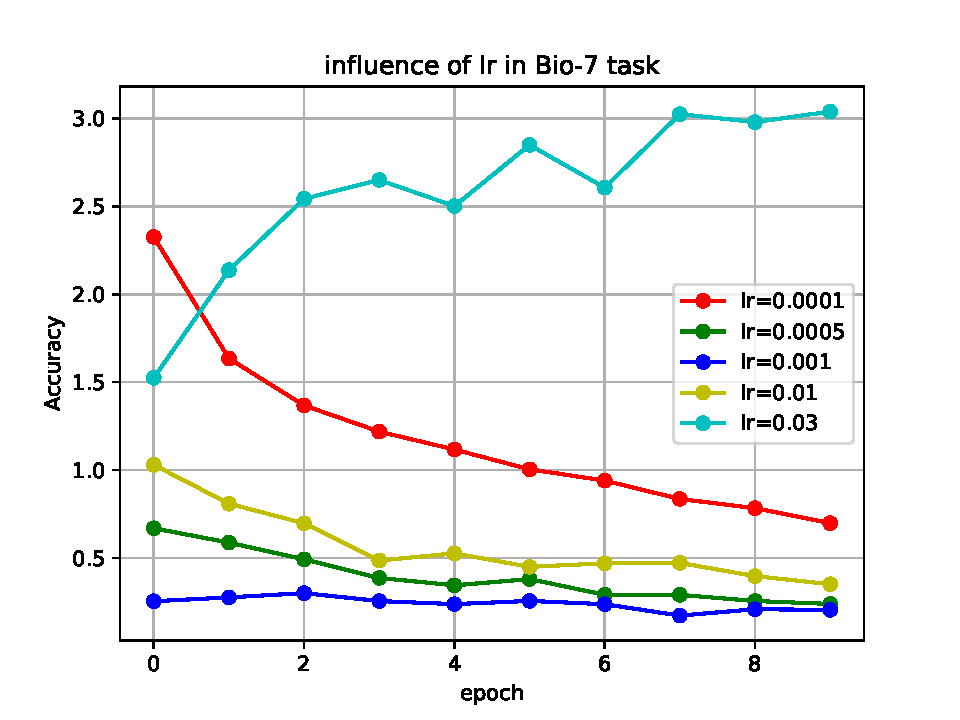
\includegraphics[width=0.24\textwidth]{../figs/lr_loss_bio.pdf}
   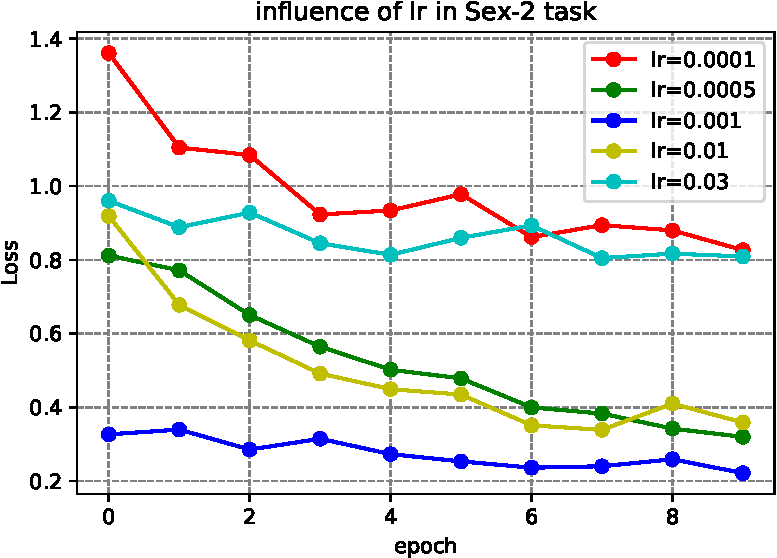
\includegraphics[width=0.24\textwidth]{../figs/lr_loss_sex.pdf}
   \caption{a.accuracy in Bio task;  b, accuracy in Sex task; c, loss in Bio task; d, loss in Sex task}
   \label{lr_result}
\centering
\end{figure}


\subsubsection{ nn on raw data}
To improve the nn' performance, we try deep neural network on  raw data. Because it is a nonlinear classifier, it may solve the relevant of raw data feature by itself. The dimension is 22283, and the network is shown in Fig{\ref{nn_1}). The setting of L2 regularization, dropout and batch normalization is same as the above experiment. But without the proper initialization (e.g. random initialization), the performance is not better than nn above. On the contrary, the accuracy is only at around 70\%, for it is easily influenced by local optimization. So we use greedy layer-wise pre training method to initialize the weights using 3 different neural network (which have the same structure as autoencoder) . Then the performance is improved a lot, besides the train process becoming faster. The best result and seleted parameters is shown in Table({\ref{nnraw_result}).\\
	
	\begin{table}[tbp]
		\centering
		\begin{tabular}{l|cccc}
			\toprule
			{Label Type} & $F_1 (\%)$ & learning rate &$batch size$  \\
			\midrule
			{\textit{MaterialType}}&99.78 & 0.001 &32\\
			{\textit{Sex}}		& 92.41 & 0.01    &50 \\
			{\textit{DiseaseState}}& 94.37 & 0.001 &32\\
			{\textit{BioSourceType}}& 98.35 & 0.001 &32\\
			\bottomrule	
		\end{tabular}
		
		\caption{Best results and parameter settings for nn model on raw data. }
		\label{nnraw_result}
	\end{table}
	
Compared with Table(\ref{nnpca_result}), it can be seen that MaterialType task and BioSourceType task has been improved, but the Sex task and DiseaseState task did not become higher. Besides, there are some differences among the optimal parameters. 

\bibliographystyle{plain}
\bibliography{report.bib}
\end{document}
